\subsubsection{Descripción y topología de los paquetes}

Nuestro primer experimento consistió en medir la LAN Wi-Fi pública del shopping Alto Palermo. Esta medición se llevó a cabo el Sábado 20 de Septiembre a las 21hs, el tiempo de medición fue de aproximádamente 40 minutos y se capturaron 1569 paquetes ARP.

Sin embargo, para graficar decidimos usar sólo los primeros 80 paquetes capturados, ya que los graficos con una cantidad tan grande de paquetes eran poco legibles.

A continuación mostramos un grafo que muestra los nodos de la red con su dirección IP y la cantidad de mensajes de tipo \emph{who-has}.

\begin{figure}[H]
 \begin{center}
  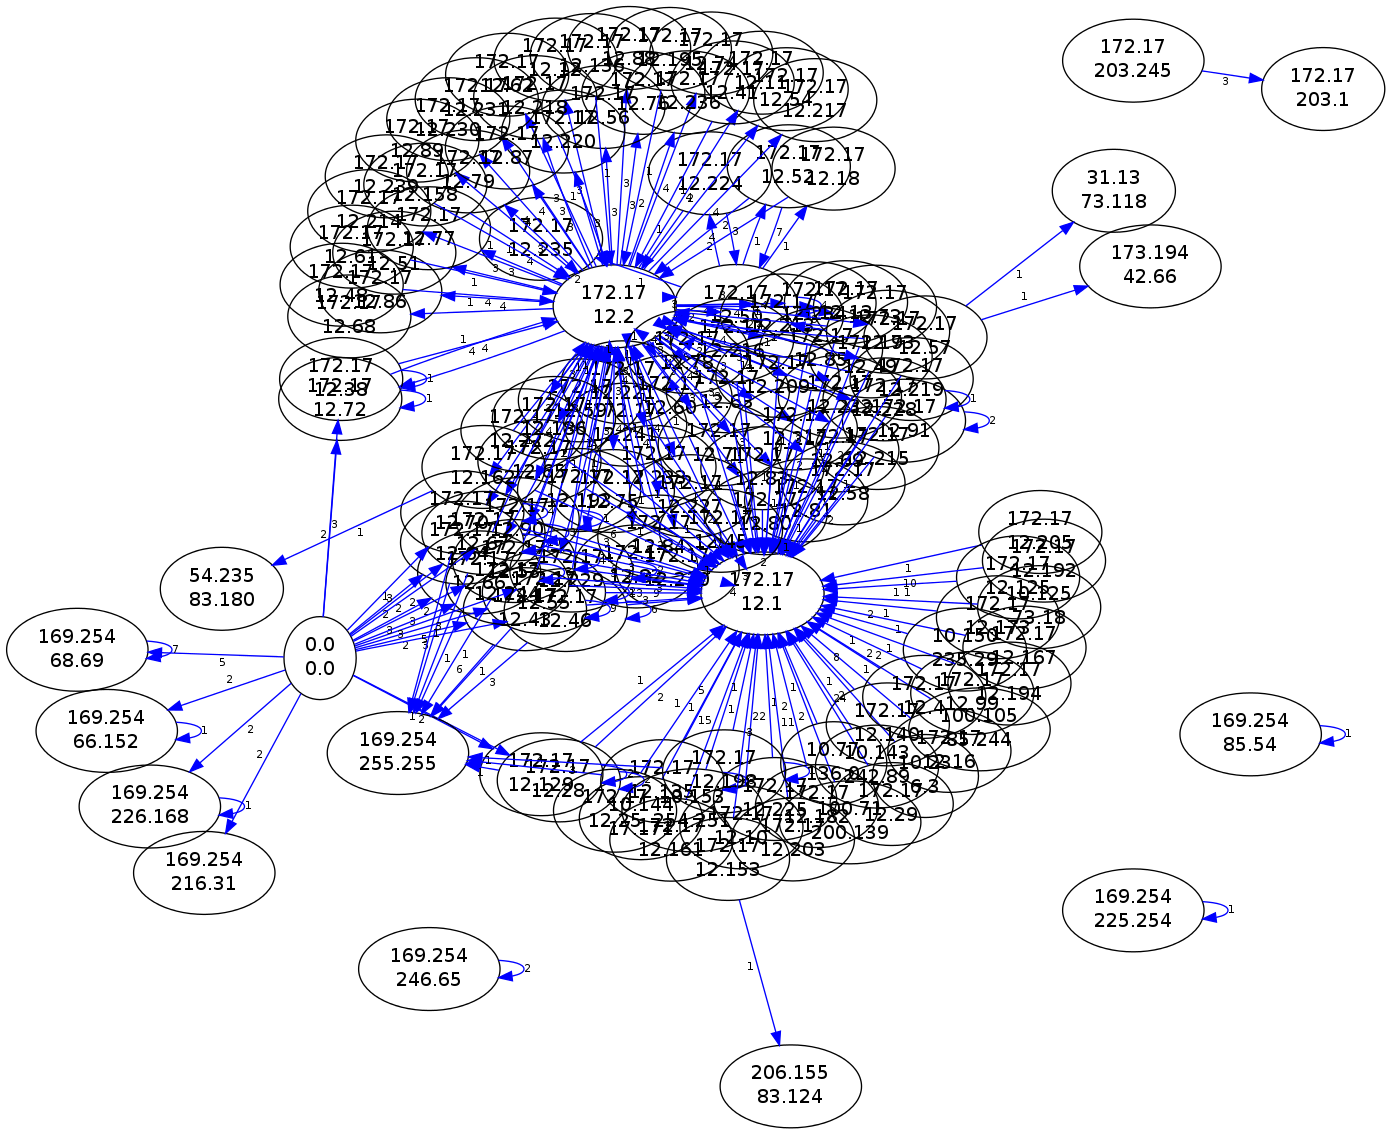
\includegraphics[width=0.9\linewidth]{../imgs/red-alto-palermo_red.png}
  \caption{Grafo Medición Alto Palermo}
 \end{center}

\end{figure}

Como podemos ver en el grafo, la red tiene dos nodos que se destacan. Uno de estos nodos, el cual tiene la dirección IP 117.17.12.1, recibe muchos paquetes de la mayoría de los otros nodos de la red, pero no envía ninguno. Y el otro recibe varios paquetes y también envía varios.

\subsubsection{Fuente: $S_{dst}$}

A continuación incluimos dos gráficos. Uno de éstos es un histograma que muestra cuántas veces apareció cada símbolo en la fuente. El otro, muestra la cantidad de información de cada símbolo de la fuente $S_{dst}$ en comparación con la entropía de la misma. 

\begin{figure}[H]\centering
    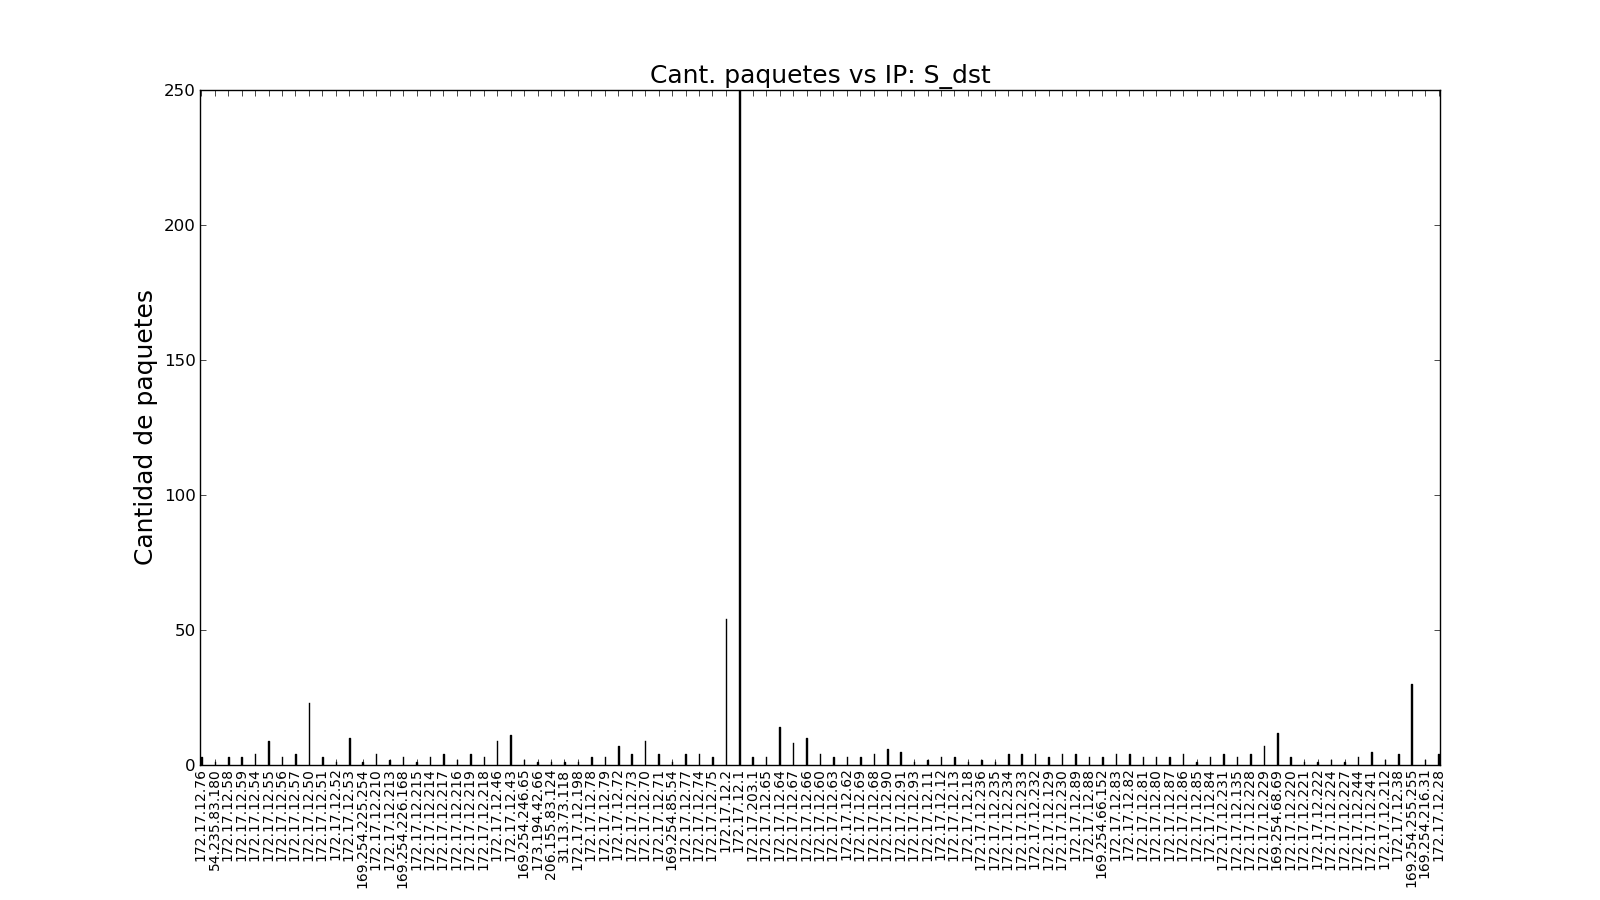
\includegraphics[width=0.8\linewidth]{../imgs/red-alto-palermo_S_dst_hist.png}
    \caption{Histograma de $S_{dst}$}\label{fig:Alto-dst-hist}
\end{figure}

\begin{figure}[H]\centering
    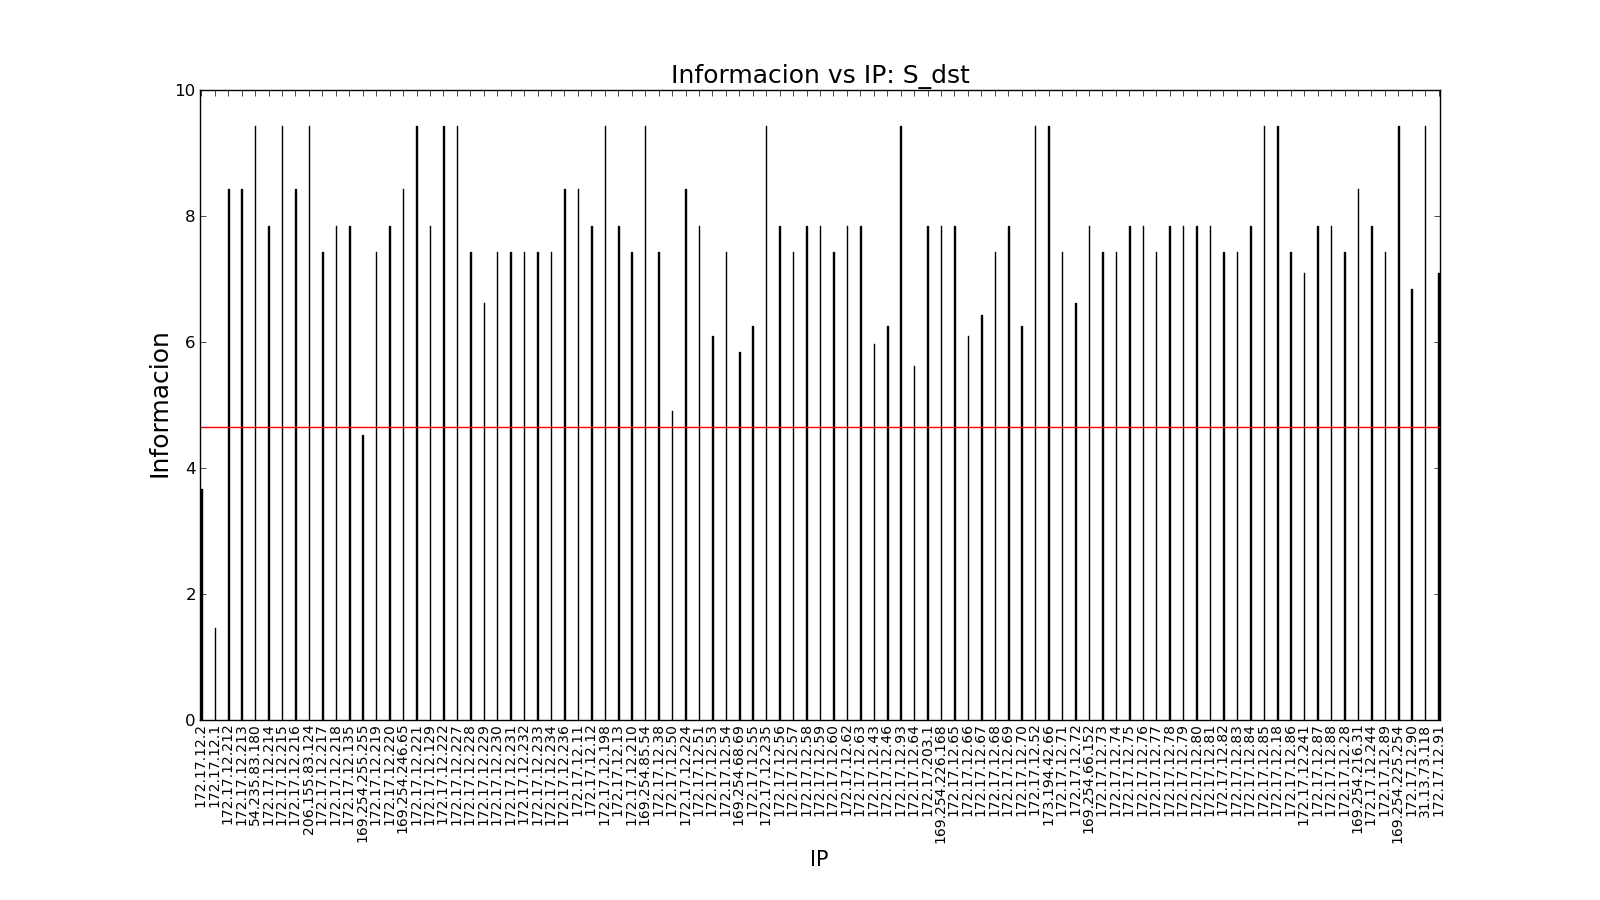
\includegraphics[width=0.8\linewidth]{../imgs/red-alto-palermo_S_dst_info.png}
    \caption{Informacion de $S_{dst}$}\label{fig:Alto-dst-info}
\end{figure}

$\bullet$ Entropía de la fuente: 4.65701881033

Como podemos observar en el primer gráfico, la dirección IP 177.17.12.1 aparece muchas más veces que el resto de las IP. Esto es así porque dicha dirección recibe mensajes de casi todos los demás nodos de la red.

En el segundo gráfico podemos ver que la cantidad de información que aporta la dirección IP 177.17.12.1 es más baja que la entopía de la fuente.
 
 
\subsubsection{Fuente: $S_{src}$}

A contincuación mostramos gráficos similares, pero esta vez para la fuente $S_{src}$:

\begin{figure}[H]\centering
    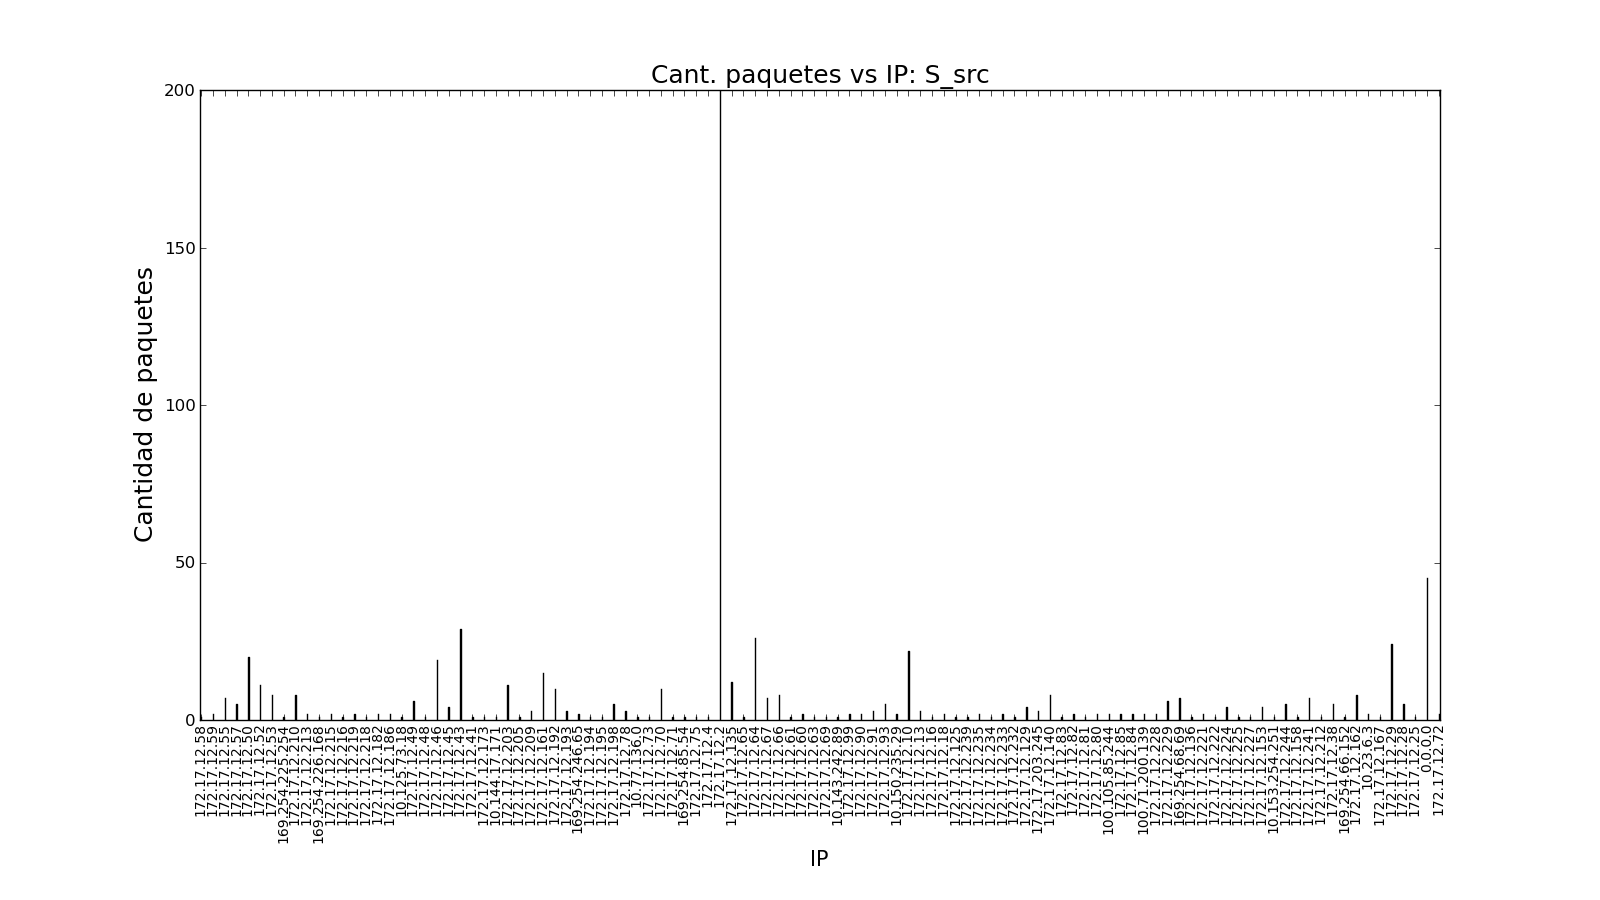
\includegraphics[width=0.8\linewidth]{../imgs/red-alto-palermo_S_src_hist.png}
    \caption{Histograma de $S_{src}$}\label{fig:Alto-src-hist}
\end{figure}

\begin{figure}[H]\centering
    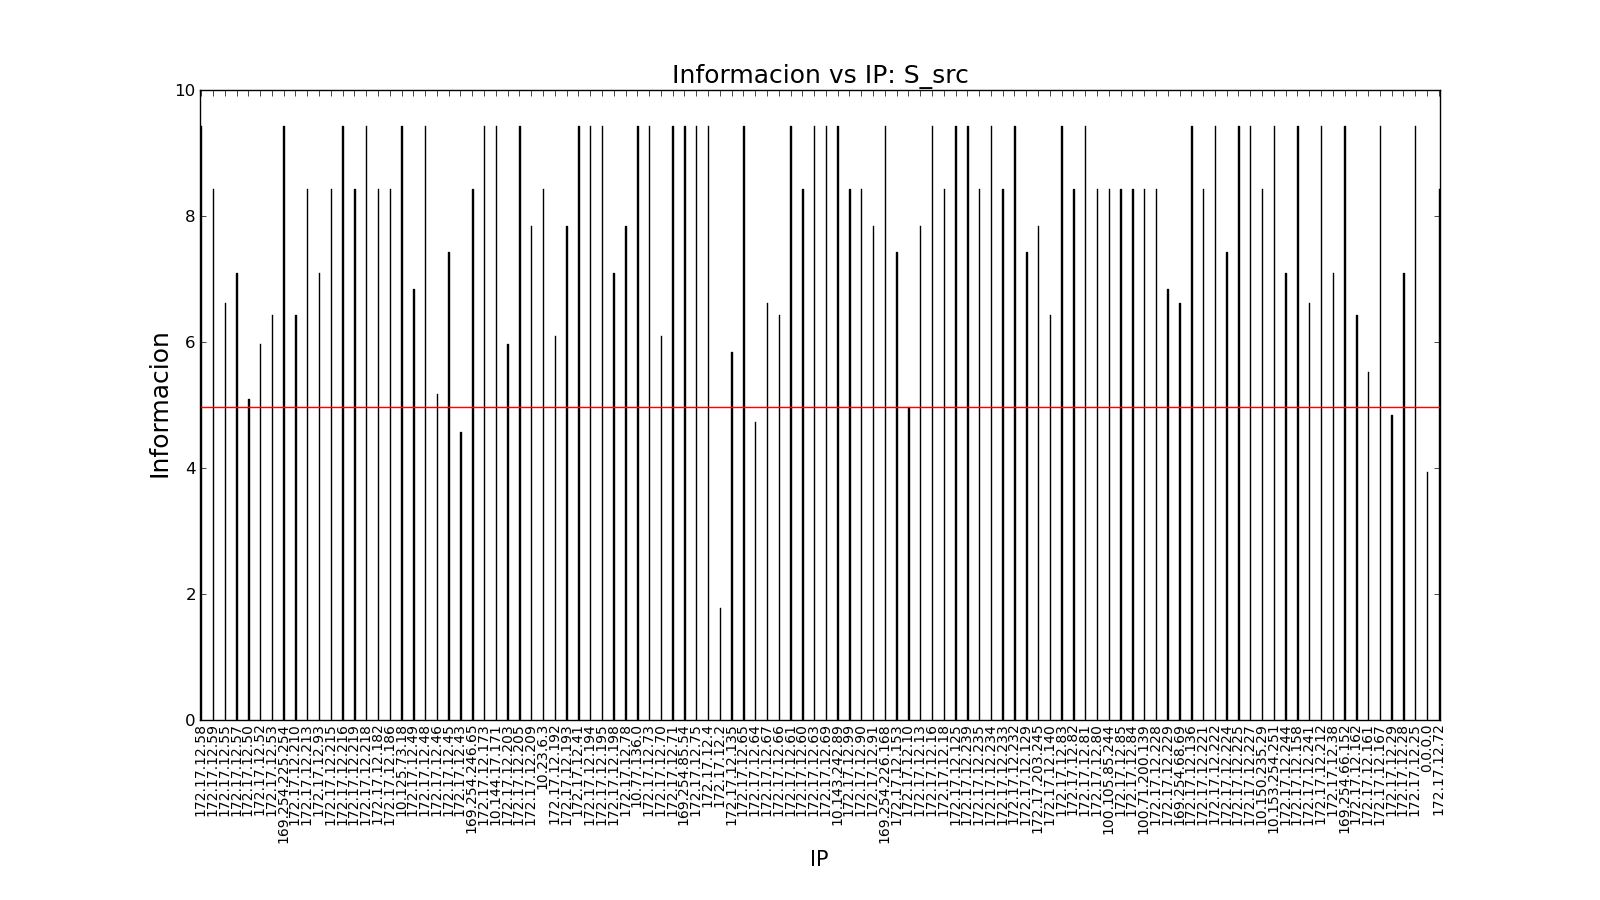
\includegraphics[width=0.8\linewidth]{../imgs/red-alto-palermo_S_src_info.png}
    \caption{Informacion de $S_{src}$}\label{fig:Alto-src-info}
\end{figure}

$\bullet$ Entropía de la fuente: 4.96088403083

En estos gráficos podemos observar que hay un nodo que envía muchos más paquetes que el resto de los nodos. Dicho nodo tiene la dirección IP 172.17.12.2. En el segundo gráfico podemos observar que la cantidad de información del símbolo 172.17.12.2 en la fuente $S_{src}$ es menor que su entropía.

Además podemos ver que hay otro nodo distinguido en esta fuente, el nodo que tiene la IP 172.17.12.135. Sin embargo, podemos ver que este nodo manda menos paquetes que el nodo 172.17.12.2.
 
\subsubsection{Discusión}

Cuando observamos el grafo en la primera parte del análisis de esta red, dijimos que había dos nodos que se destacaban visualmente, los cuales eran los que tenían las direcciones IP 177.17.12.1 y 177.17.12.2. Al ver el grafo notamos que la mayor parte de los paquetes capturados eran enviados o recibidos por alguno de estos dos nodos. Esto nos hizo suponer que éstos eran los dos nodos distinguidos de la red.

Al luego observamos el histograma y el gráfico de barras de la fuente $S_{dst}$. De esta forma vimos que efectivamente el nodo con la IP 117.17.12.1 aparecía como dirección destino en muchos mensajes. Sin embargo el nodo 177.17.12.2 no aparecía tantaas veces.

Luego de hacer lo mismo con la fuente $S_{src}$ notamos que el nodo que aparecía más veces era el nodo 177.17.12.2. El nodo 177.17.12.1 no era un símbolo de $S_{src}$ ya que éste no mando mensajes, por lo tanto no aparece en estos gráficos.

Concluimos entonces que el nodo de la red que tiene la dirección IP 177.17.12.1 se trata de un nodo distinguido, el cual creemos que es el router de la red. Sin embargo, no pudimos ver qué rol ocupaba el nodo 177.17.12.2 en la misma.